% 05-Metodologia_Presentacion_Tesis.tex
% Diapositivas de la sección Metodología

\section{Metodología}

\begin{frame}
\frametitle{Flujo General de la Metodología}
\begin{itemize}
    \item Desarrollo de modelos de aprendizaje profundo para la detección de 15 patologías pulmonares en rayos X.
    \item Dos enfoques principales: ResNet50 (CNN) y Vision Transformer (ViT).
    \item Proceso estructurado: preprocesamiento, entrenamiento, evaluación y extensión a nuevas patologías.
\end{itemize}
\end{frame}

\begin{frame}
\frametitle{Bases de Datos y Composición}
\begin{itemize}
    \item Uso del dataset ChestX-ray14 (112,120 imágenes, 30,805 pacientes, 14 patologías).
    \item Extensión con imágenes de COVID-19 y saludables.
    \item Re-etiquetado de datos usando modelos automáticos para mejorar la calidad de las etiquetas.
\end{itemize}
\end{frame}

\begin{frame}
\frametitle{Preprocesamiento de Imágenes}
\begin{itemize}
    \item Redimensionamiento a $1024 \times 1024$ y $384 \times 384$ píxeles según el modelo.
    \item Normalización y estandarización de intensidades.
    \item Data augmentation: rotaciones, traslaciones, escalados y flips para robustez.
\end{itemize}
\end{frame}

\begin{frame}
\frametitle{Entrenamiento: Transfer Learning y Fine-Tuning}
\begin{itemize}
    \item ResNet50 y ViT preentrenados en ImageNet.
    \item Tres etapas: (1) Transfer learning (cambio de la capa de salida), (2) Fine-tuning de las últimas capas, (3) Full-tuning de toda la red.
    \item Permite adaptar modelos generales a tareas médicas específicas con menos datos.
\end{itemize}
\end{frame}

\begin{frame}
\frametitle{Arquitectura de los Modelos}
\begin{columns}
\column{0.5\textwidth}
\textbf{ResNet50}
\begin{itemize}
    \item Red convolucional profunda con conexiones residuales.
    \item Extrae características espaciales de las radiografías.
\end{itemize}
\column{0.5\textwidth}
\textbf{Vision Transformer (ViT)}
\begin{itemize}
    \item Divide la imagen en parches y los procesa como una secuencia.
    \item Utiliza mecanismos de atención para capturar relaciones globales.
\end{itemize}
\end{columns}
\begin{figure}[ht!]
    \centering
    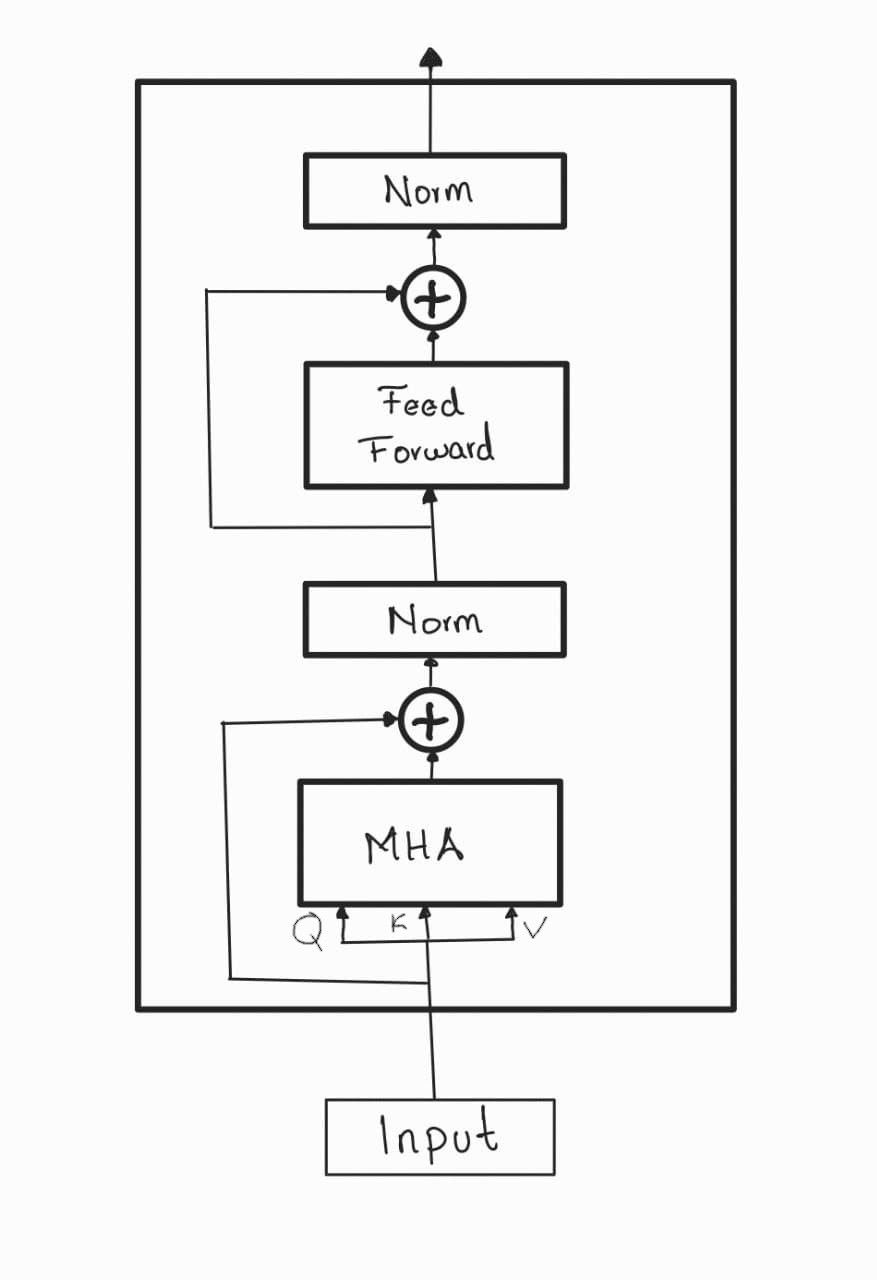
\includegraphics[width=0.5\textwidth]{../Chapters/2. Transformer/Figures/transformer/encoder.jpg}
    \caption{Esquema de codificador Transformer (ViT).}
\end{figure}
\end{frame}

\begin{frame}
\frametitle{Evaluación y Métricas}
\begin{itemize}
    \item División de datos en entrenamiento, validación y prueba.
    \item Métricas: AUC, precisión, recall, F1-score y matriz de confusión.
    \item Visualización de resultados: mapas de calor y curvas ROC.
\end{itemize}
\begin{figure}[ht!]
    \centering
    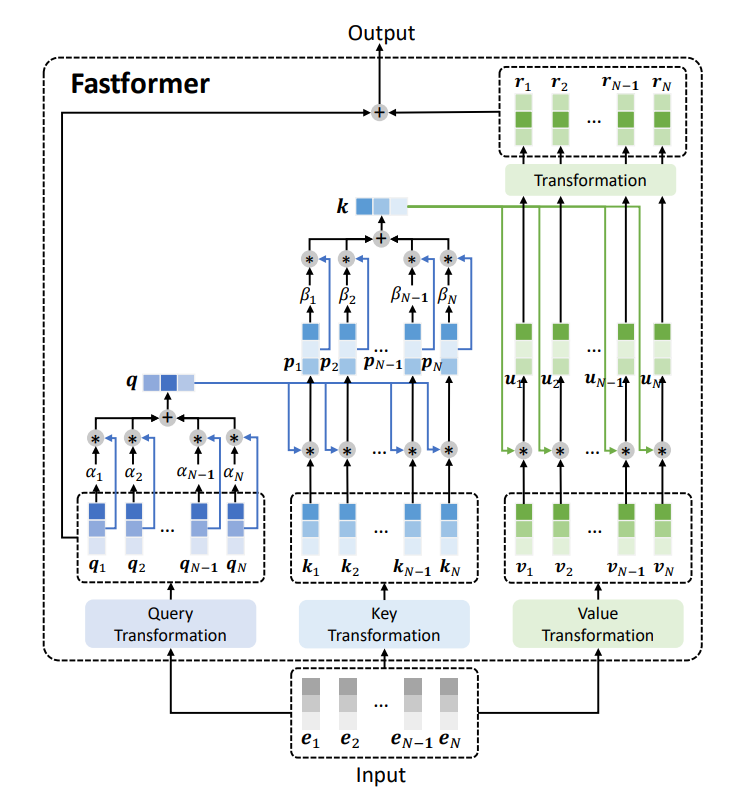
\includegraphics[width=0.3\textwidth]{../Chapters/2. Transformer/Figures/transformer/fastformer.png}
    \caption{Ejemplo de visualización de atención en modelos tipo Transformer.}
\end{figure}
\end{frame}

\begin{frame}
\frametitle{Extensión y Generalización}
\begin{itemize}
    \item El modelo puede ser extendido fácilmente a nuevas patologías (ejemplo: tuberculosis).
    \item El proceso de re-etiquetado y entrenamiento permite adaptar el sistema a diferentes escenarios clínicos.
    \item Resultados competitivos frente al estado del arte en todas las patologías evaluadas.
\end{itemize}
\end{frame}
